%%%%%%%%%%%%%%%%%%%%%%%%%%%%%%%%%%%%%%%%%%%%%%%%%%%%%%%%%%%%%%%%%%%%%%%%%%%%%%%%
%% SUBSECTION: Metodologia badania
%%%%%%%%%%%%%%%%%%%%%%%%%%%%%%%%%%%%%%%%%%%%%%%%%%%%%%%%%%%%%%%%%%%%%%%%%%%%%%%%
\subsection{Metodologia badania}


\begin{equation} \label{energy_equation}
E_{\text{całkowita}} = U \cdot \int_{t=0[s]}^{t=50[s]} \mathrm{d}i \: \mathrm{d} t
\end{equation}

\begin{equation} \label{power_equation}
P = \frac{E_{\text{całkowita}}}{t}
\end{equation}

gdzie:

\begin{description}
\item $E_{\text{całkowita}} [J]$ - energia zużyta podczas 50s sekundowej sesji rejestracji danych
\item $P [W]$ - mocz użyta podczas 50s sekundowej sesji rejestracji danych
\item $U [V]$ - napięcie zasilania mikrokontrolera - 3.3V
\item $\mathrm{d}i [A]$ - prąd w danej chwili
\item $\mathrm{d}t [s]$ - podstawa czasowa całkowania, 0.01s/interwał (100Hz)
\end{description}


\lipsum[1-3]
%%%%%%%%%%%%%%%%%%%%%%%%%%%%%%%%%%%%%%%%%%%%%%%%%%%%%%%%%%%%%%%%%%%%%%%%%%%%%%%%
%% SUBSECTION: BT Low Energy - Usługa Heart Rate
%%%%%%%%%%%%%%%%%%%%%%%%%%%%%%%%%%%%%%%%%%%%%%%%%%%%%%%%%%%%%%%%%%%%%%%%%%%%%%%%
\subsection{BT Low Energy - Usługa Heart Rate}

\lipsum[1-3]
\begin{figure}[!htb]
	\centering 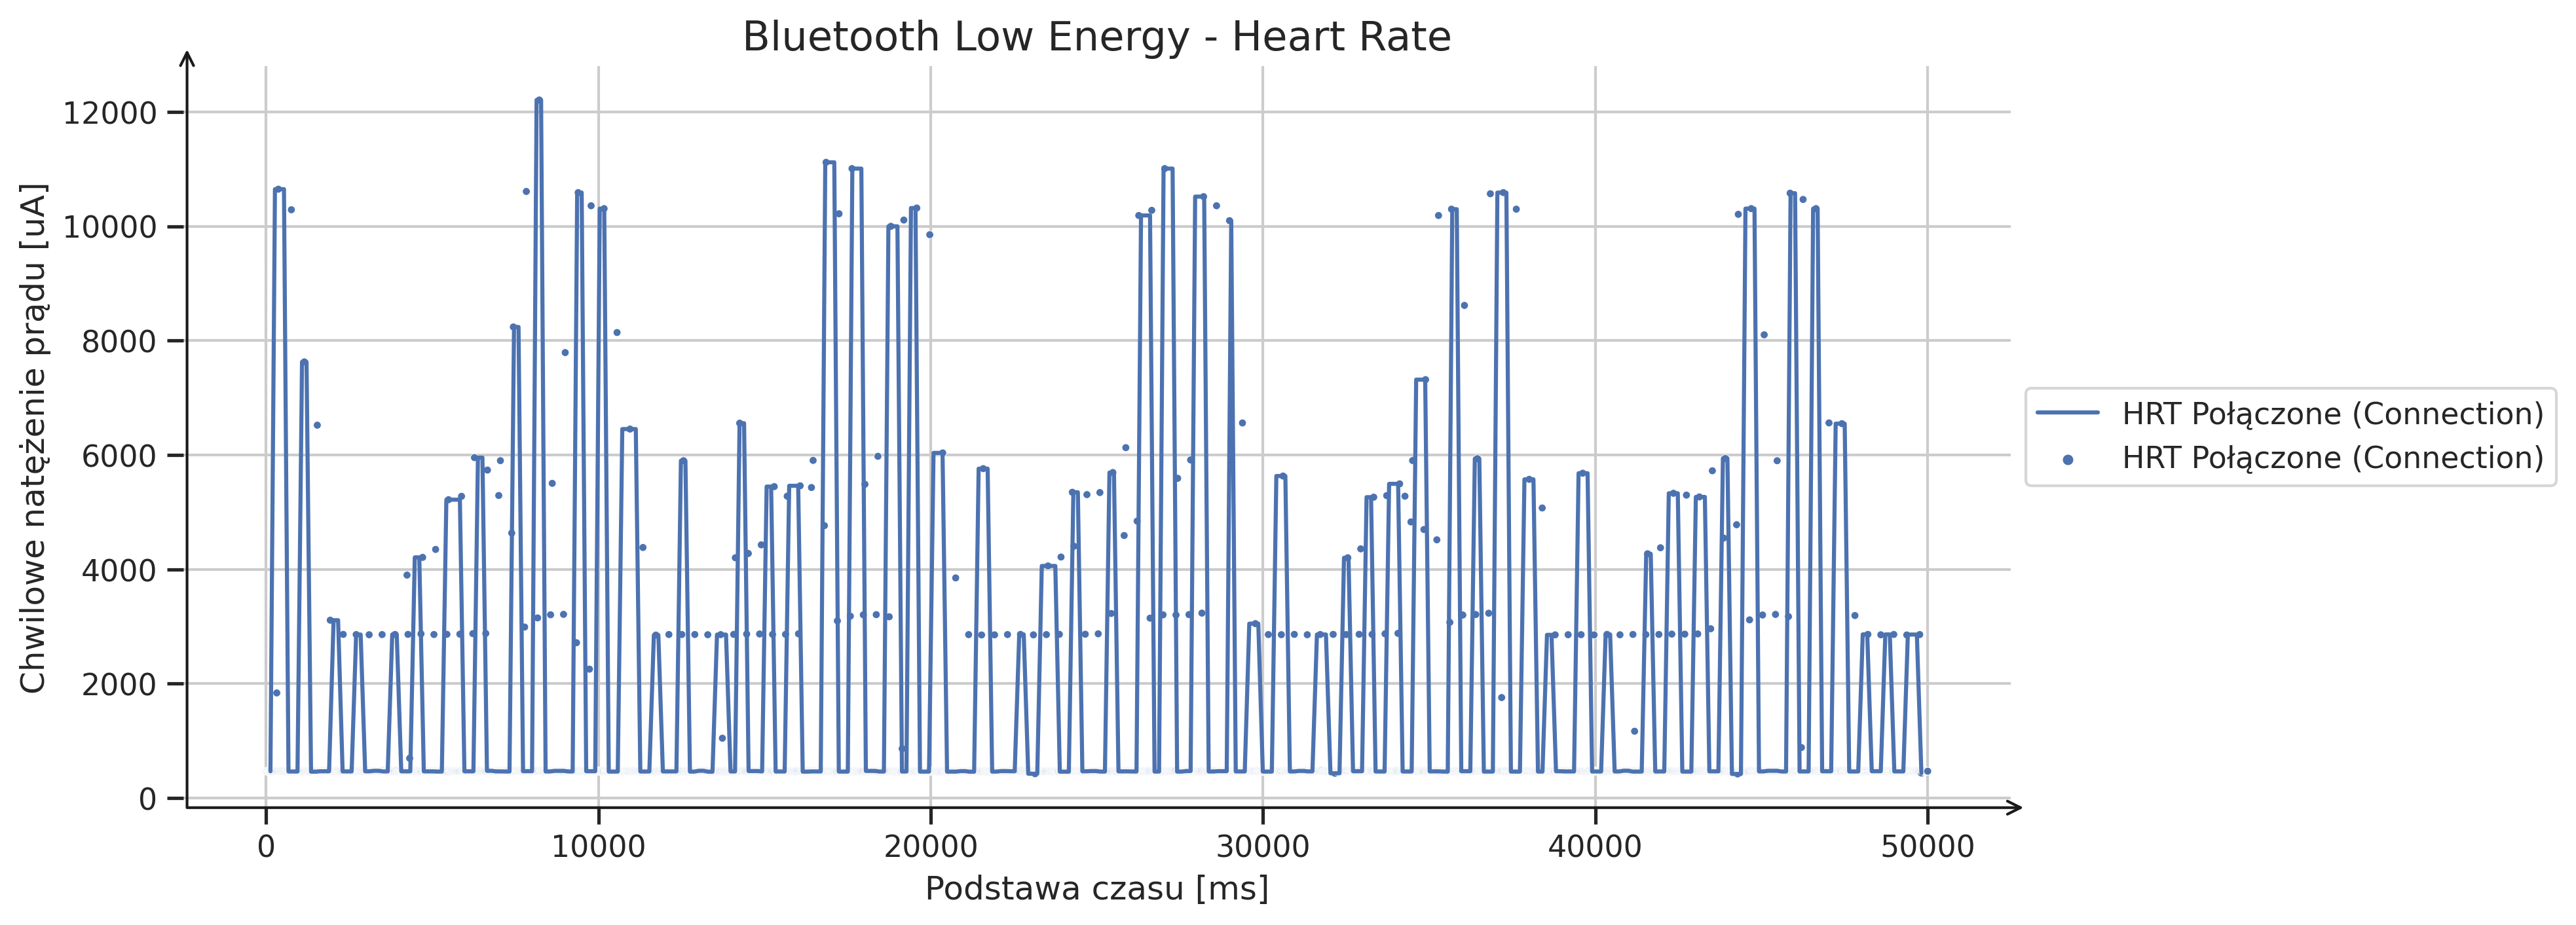
\includegraphics[width=0.99\linewidth]{power_ble_hr_connected_only_amps.png}
	\caption{Charakterystyka czasowa poboru prądu dla BLE i usługi Heart Rate - Usługa Połączona}
	\label{rys:power_ble_hr_connected_only_amps}
\end{figure}

\lipsum[1-3]
\begin{figure}[!htb]
	\centering 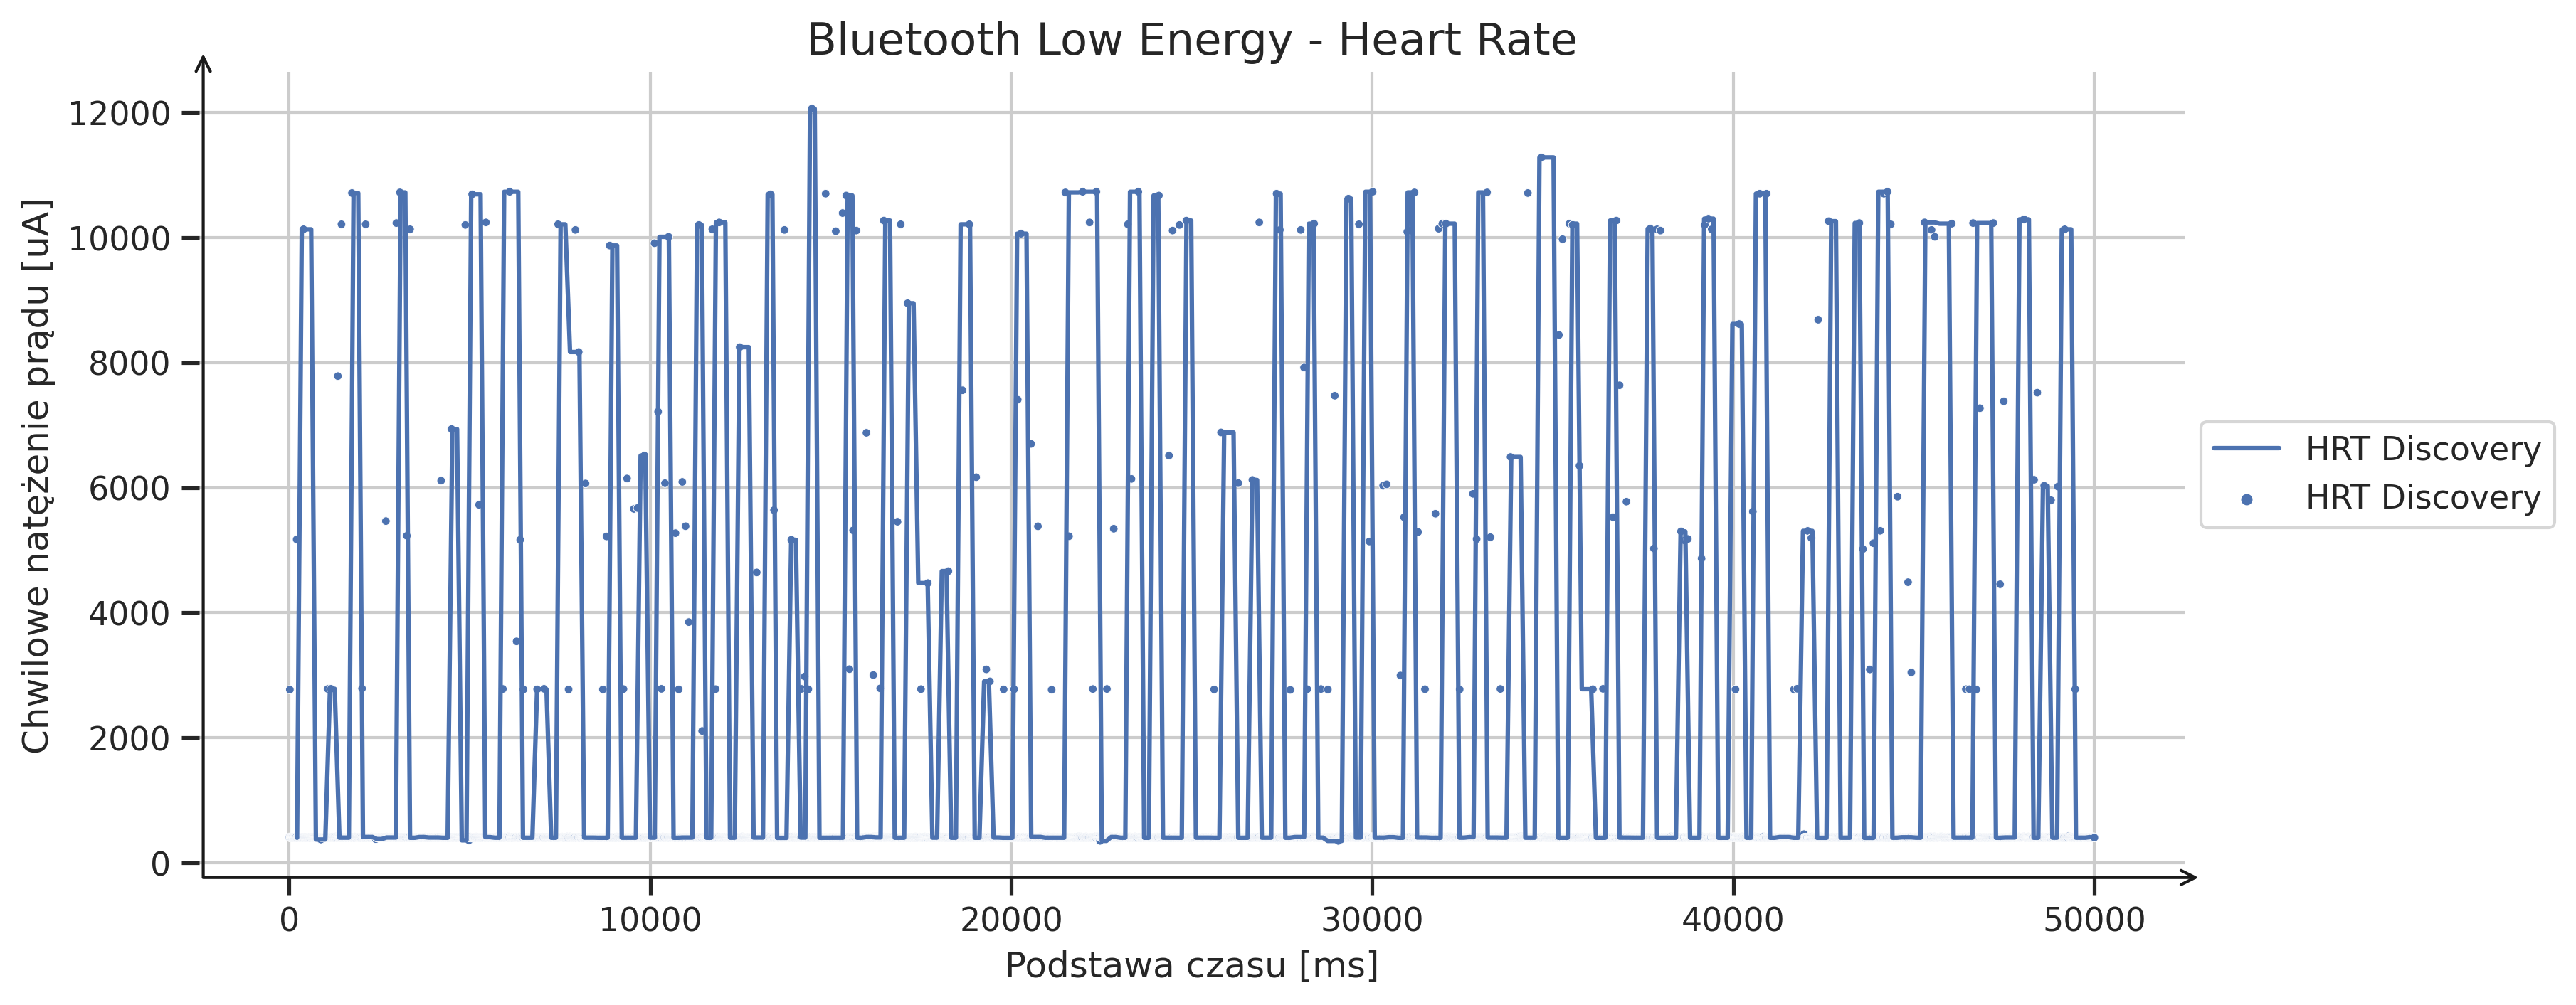
\includegraphics[width=0.99\linewidth]{power_ble_hr_discovery_only_amps.png}
	\caption{Charakterystyka czasowa poboru prądu dla BLE i usługi Heart Rate - Wyszukiwanie}
	\label{rys:power_ble_hr_discovery_only_amps}
\end{figure}

\lipsum[1-3]
\begin{figure}[!htb]
	\centering 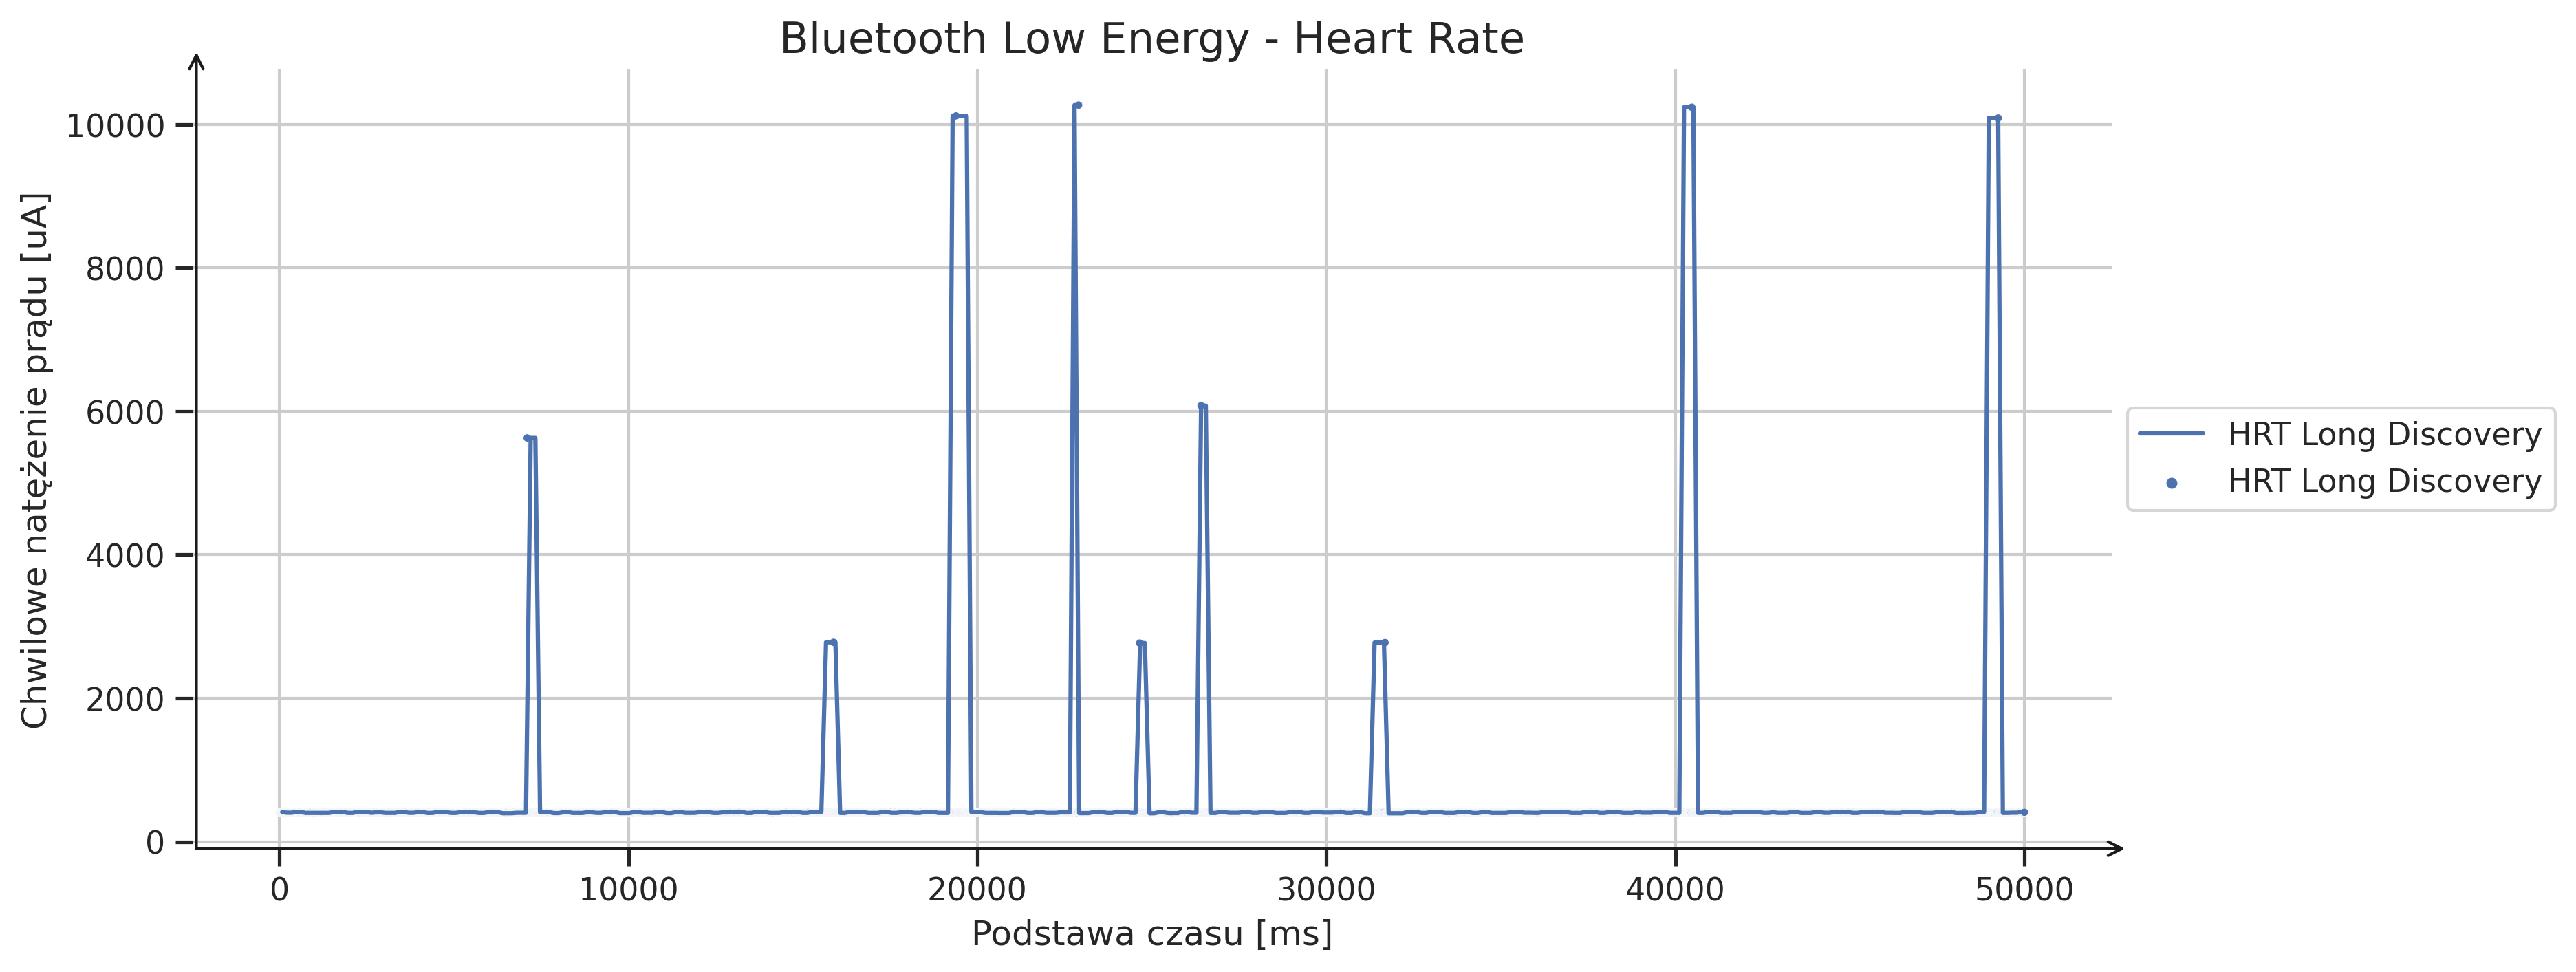
\includegraphics[width=0.99\linewidth]{power_ble_hr_long_connected_only_amps.png}
	\caption{Charakterystyka czasowa poboru prądu dla BLE i usługi Heart Rate - Wyszukiwanie, urządzenie w gotowości}
	\label{rys:power_ble_hr_long_connected_only_amps}
\end{figure}


\lipsum[1-2]
\begin{figure}[!htb]
	\centering 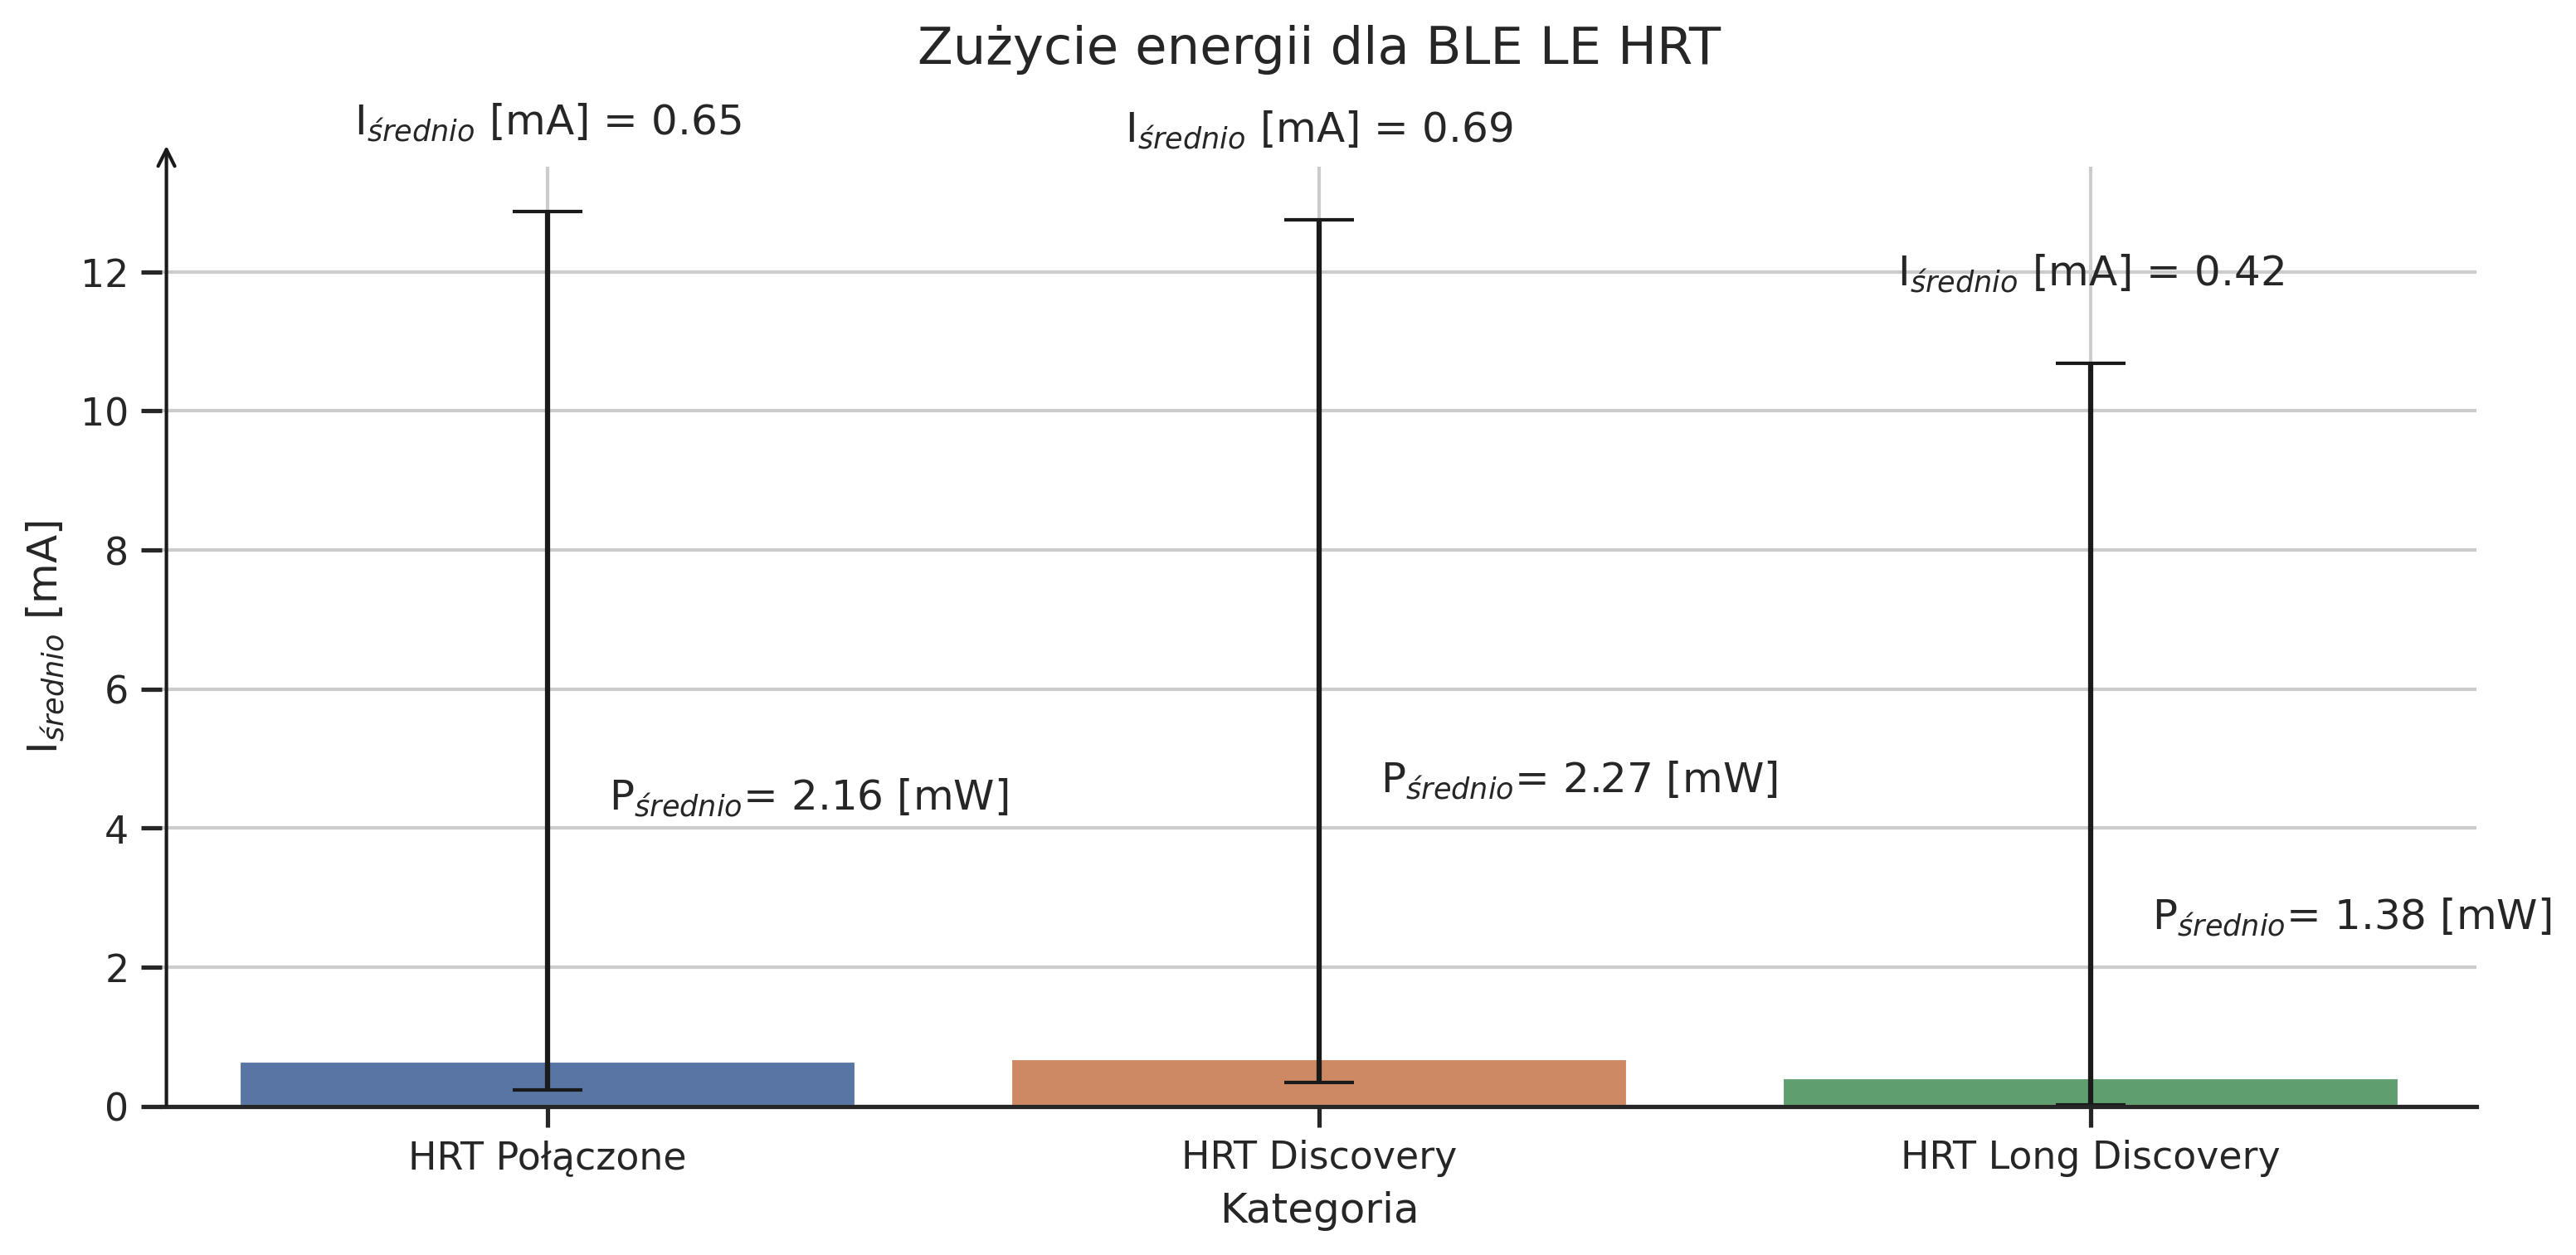
\includegraphics[width=0.99\linewidth]{power_ble_hr_amps_usage_juxtaposition.png}
	\caption{Zestawienie zużycia prądu dla usługi Heart Rate w zależności od trybu działania}
	\label{rys:power_ble_hr_amps_usage_juxtaposition}
\end{figure}
\lipsum[1-3]

%%%%%%%%%%%%%%%%%%%%%%%%%%%%%%%%%%%%%%%%%%%%%%%%%%%%%%%%%%%%%%%%%%%%%%%%%%%%%%%%
%% SUBSECTION: BLE Mesh - Model Generic OnOff
%%%%%%%%%%%%%%%%%%%%%%%%%%%%%%%%%%%%%%%%%%%%%%%%%%%%%%%%%%%%%%%%%%%%%%%%%%%%%%%%
\subsection{BLE Mesh - Model Generic OnOff}

Pomiary dla BLE Mesh uwzględniające dwa tryby działania: sieć w oczekująca na komunikaty oraz podczas działania aktywnego korzystania z Modelu Generic OnOff.

\begin{figure}[!htb]
	\centering 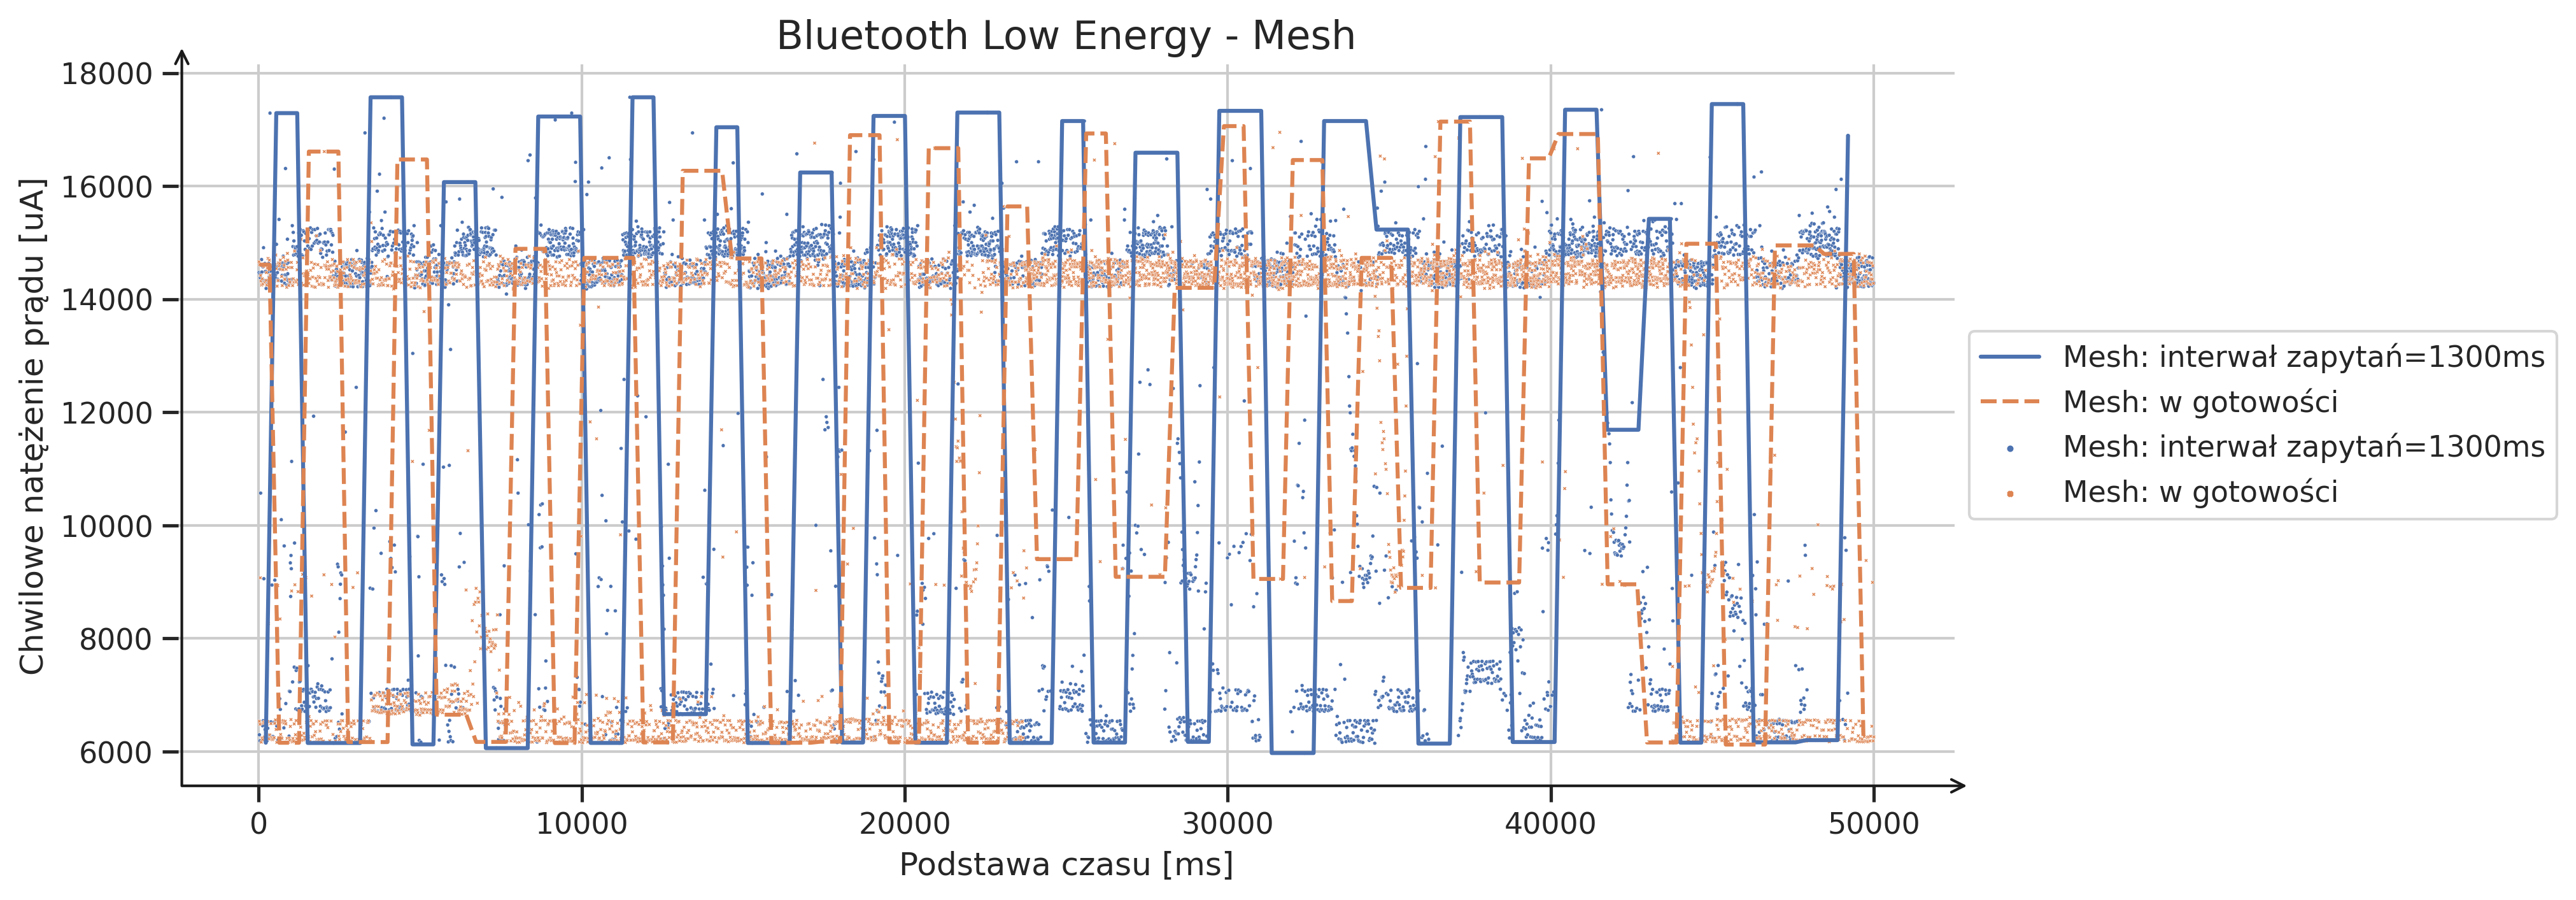
\includegraphics[width=0.99\linewidth]{power_ble_mesh_amps.png} 
	\caption{Charakterystyka czasowa poboru prądu dla BLE Mesh i modelu Generic OnOff}
	\label{rys:power_ble_mesh_amps}
\end{figure}

\lipsum[1-3]
\begin{figure}[!htb]
	\centering 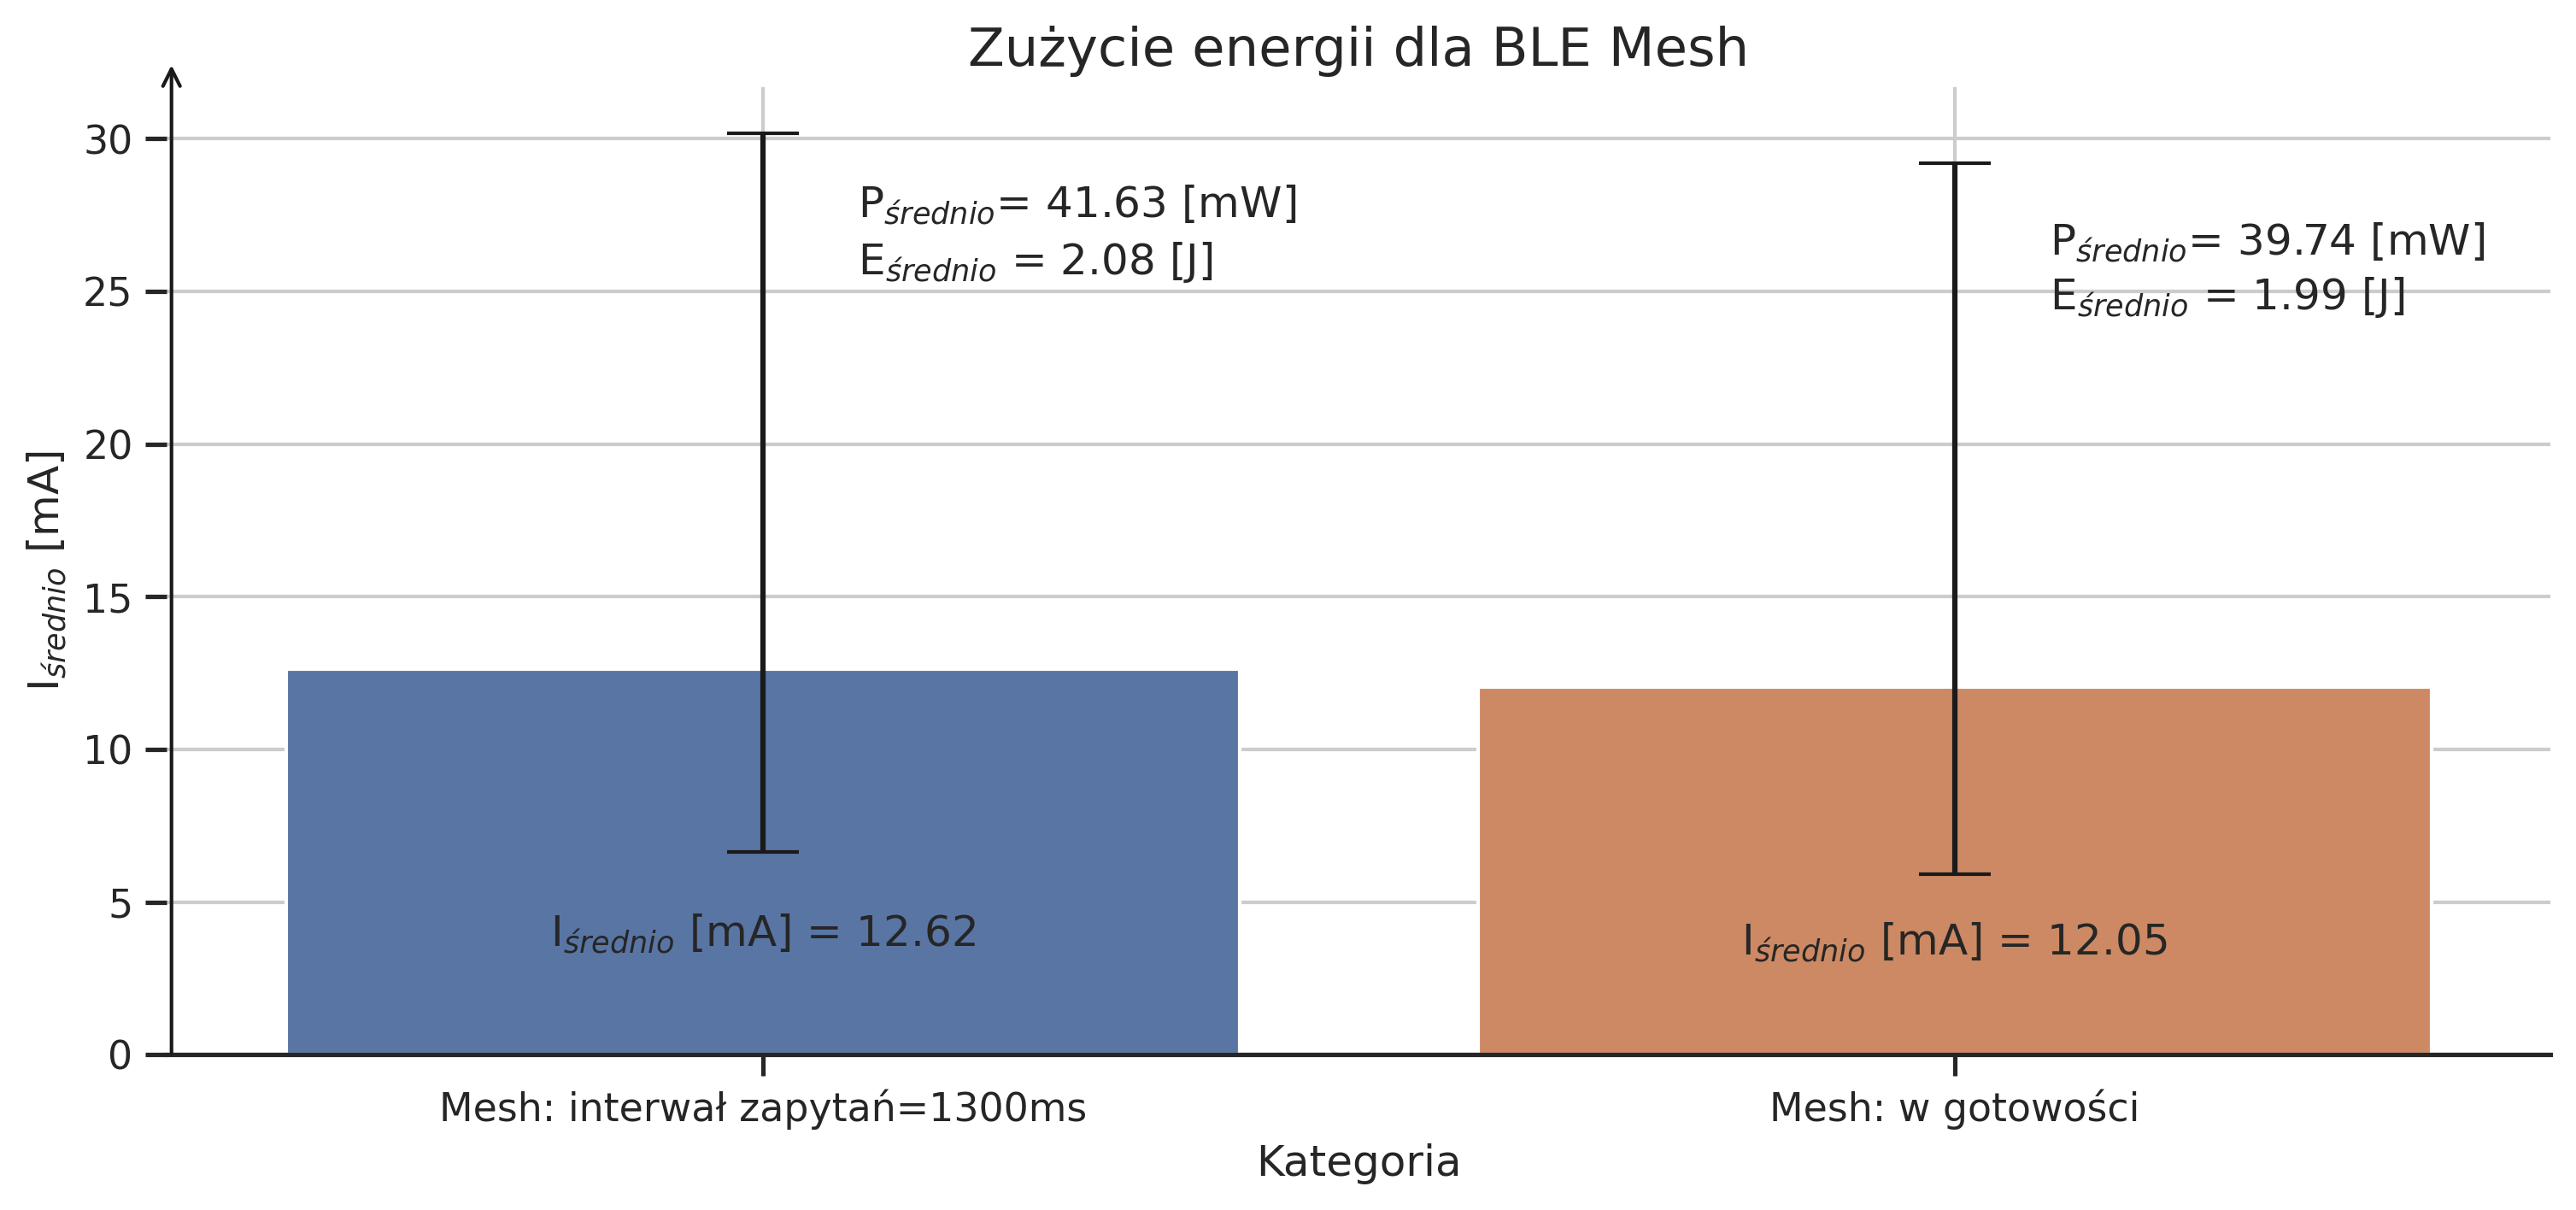
\includegraphics[width=0.99\linewidth]{power_ble_mesh_amps_usage_juxtaposition.png} 
	\caption{Zestawienie zużycia prądu dla BLE Mesh w zależności od trybu działania}
	\label{rys:power_ble_mesh_amps_usage_juxtaposition}
\end{figure}

\lipsum[1-3]
\begin{figure}[!htb]
	\centering 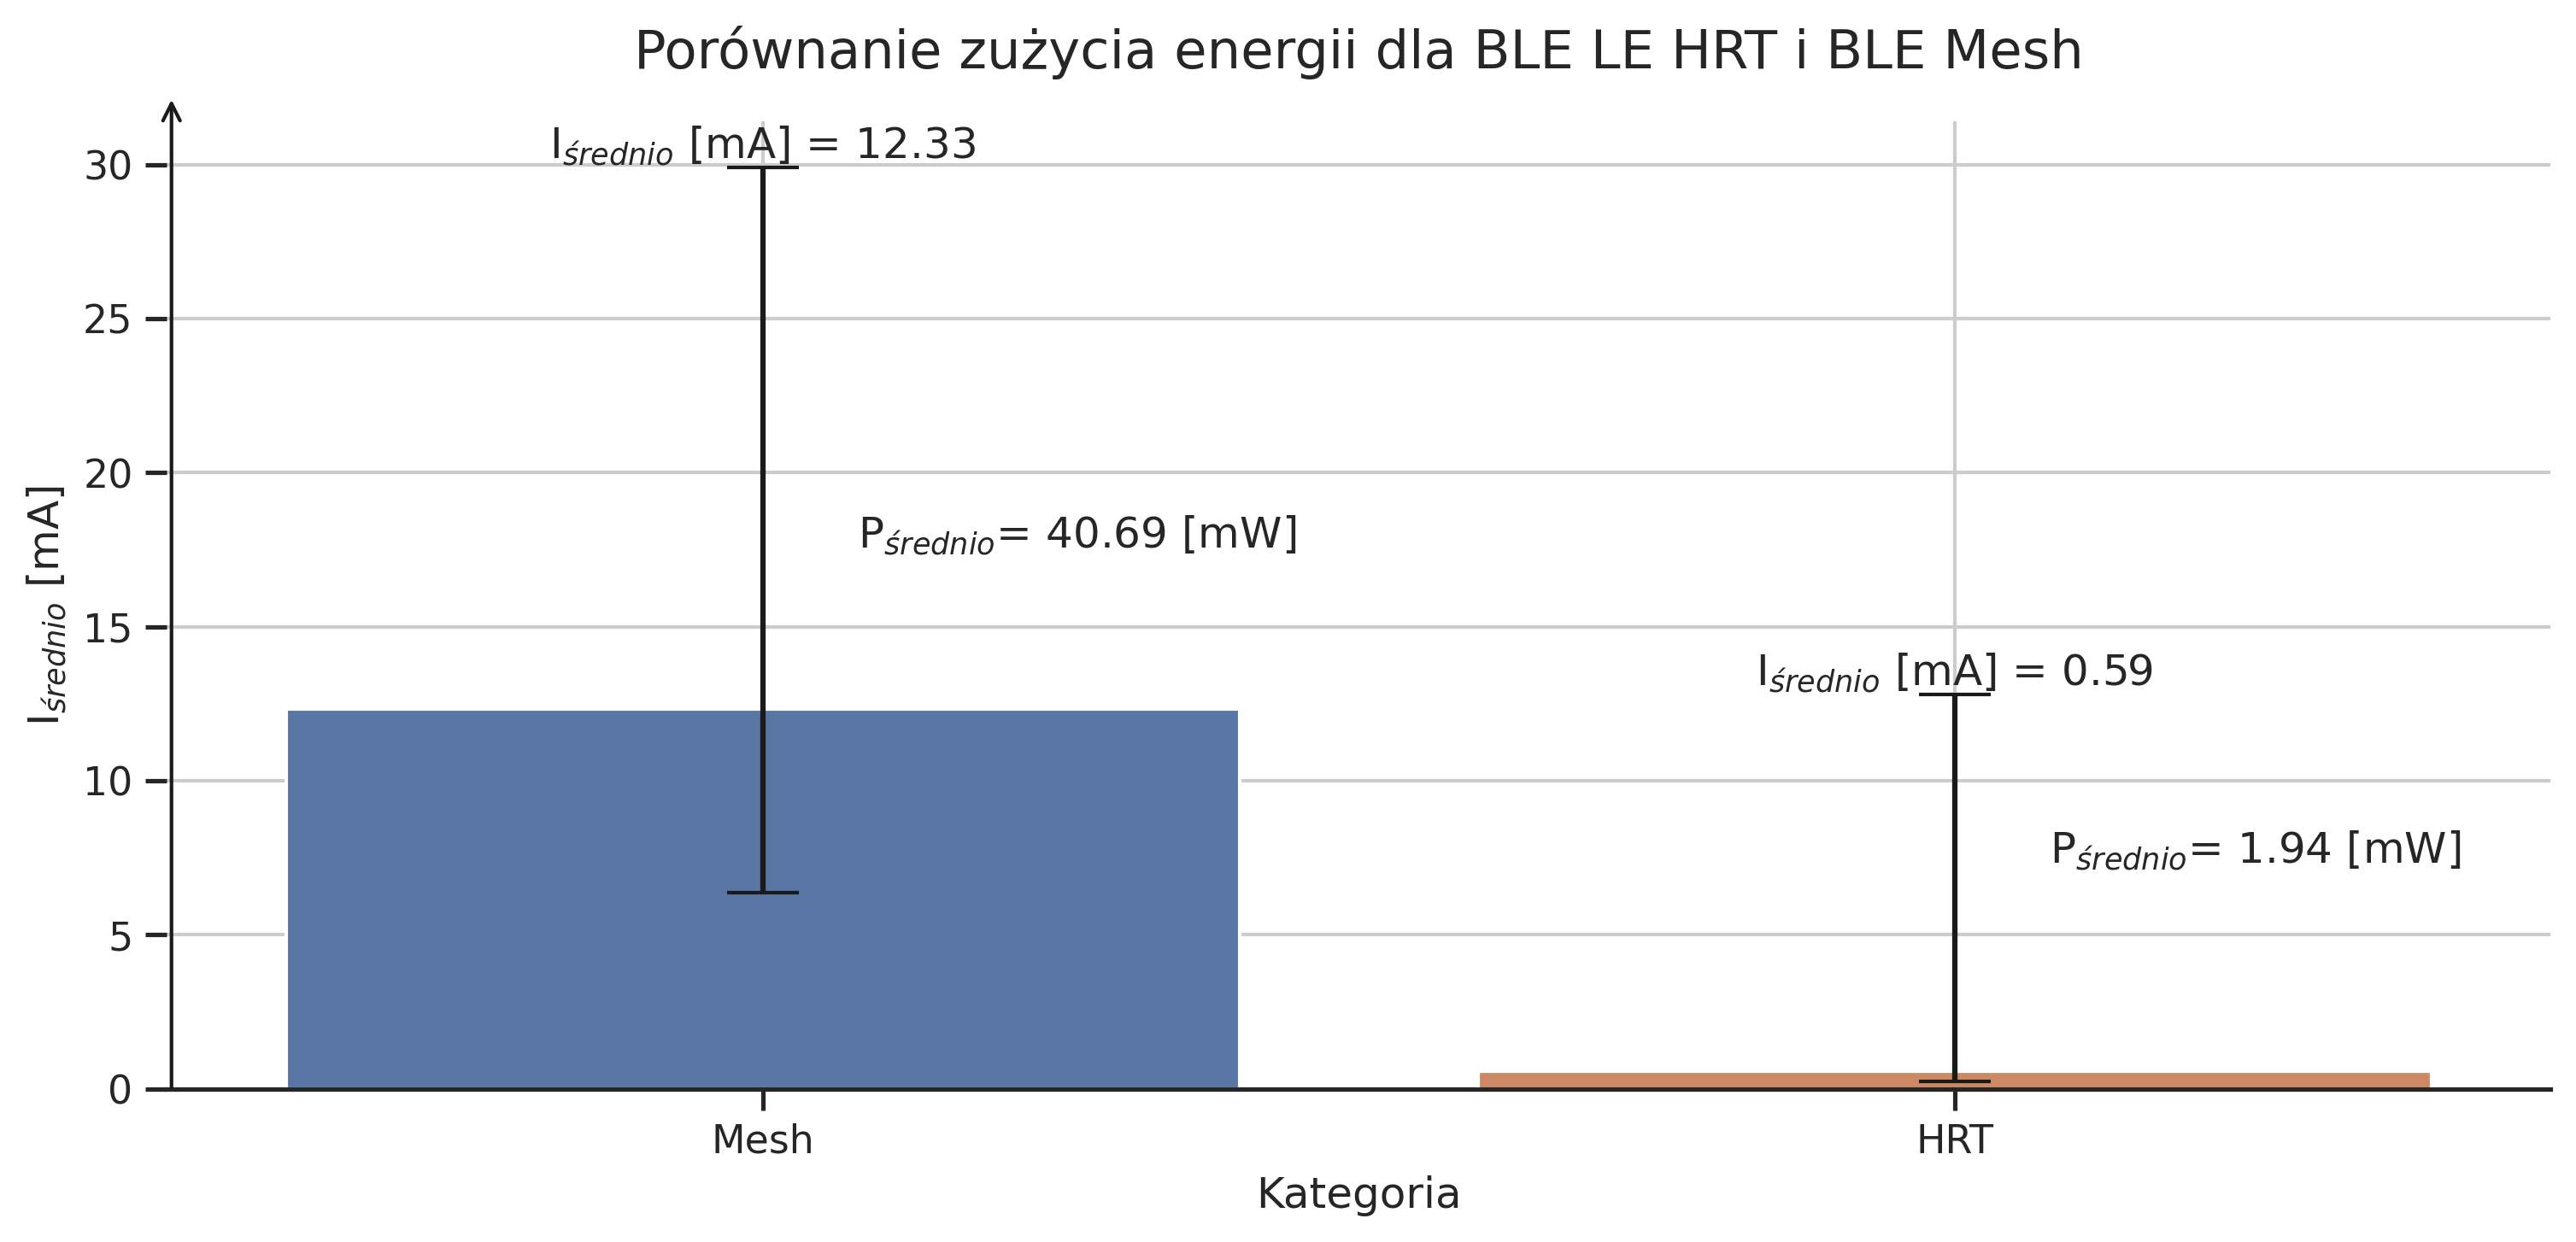
\includegraphics[width=0.99\linewidth]{power_ble_consumption_comparison.png} 
	\caption{Porównanie średniego zużycia energii pomiędzy BT Low Energy HRT i BLE Mesh}
	\label{rys:power_ble_consumption_comparison}
\end{figure}


